\chapter{Visualizing Data}\label{s:vis}

Tables and lists are great, but visualizations are often more effective---if
they're well designed and your audience is sighted, that is.
There are even more ways to visualize data in the browser
than there are front-end toolkits for JavaScript.
We have chosen to use \href{http://vega.github.io/}{Vega-Lite},
which is a \gref{g:declarative}{declarative} framework:
as a user,
you specify the data and settings,
and let the library take care of everything else.
It doesn't do everything,
but it does common things well and easily,
and it interacts nicely with React.

\section{Vega-Lite}\label{s:vis-vega-lite}

Let's start by creating a skeleton web page to hold our visualization.
For now, we will load Vega, Vega-Lite, and Vega-Embed from the web;
we'll worry about local installation later.
We will create a \texttt{div} to be filled in by the visualization---we
don't have to give it the ID \texttt{vis}, but it's common to do so---and
we will leave space for the script.
Our skeleton looks like this
(with lines broken for the benefit of the printed version):

\begin{minted}{html}
<!DOCTYPE html>
<html>
<head>
  <title>Embedding Vega-Lite</title>
  <script src="https://cdn.jsdelivr.net/npm/vega@5"></script>
  <script src="https://cdn.jsdelivr.net/npm/vega-lite@3"></script>
  <script src="https://cdn.jsdelivr.net/npm/vega-embed@4"></script>
</head>
<body>

  <div id="vis"></div>

  <script type="text/javascript">
  </script>
</body>
</html>
\end{minted}

We can now start filling in the script with the beginning of a visualization specification.
This is a blob of \gref{g:json}{JSON} with certain required fields:

\begin{itemize}
\item
  \texttt{\$schema} identifies the version of the spec being used (as a URL).
\item
  \texttt{description} is a comment to remind us what we thought we were doing when we created this.
\item
  \texttt{data} is the actual data.
\end{itemize}

\begin{minted}{html}
...rest of page as before...
  <script type="text/javascript">
    let spec = {
      "$schema": "https://vega.github.io/schema/vega-lite/v2.0.json",
      "description": "Create data array but do not display anything.",
      "data": {
        "values": [
          {"a": "A", "b": 28},
          {"a": "B", "b": 55},
          {"a": "C", "b": 43},
          {"a": "D", "b": 91},
          {"a": "E", "b": 81},
          {"a": "F", "b": 53},
          {"a": "G", "b": 19},
          {"a": "H", "b": 87},
          {"a": "I", "b": 52}
        ]
      }
    }
  </script>
...rest of page as before...
\end{minted}

In this case,
we represent a two-dimensional data table as objects with explicit indices \texttt{"a"} and \texttt{"b"}.
We have to do this because JSON (like JavaScript) doesn't have a native representation
of two-dimensional arrays with row and column headers,
because programmers.

Once we have created our spec,
we can call \texttt{vegaEmbed} with the ID of the element that will hold the visualization,
the spec,
and some options (which for now we will leave empty):

\begin{minted}{js}
    let spec = {
      "$schema": "https://vega.github.io/schema/vega-lite/v2.0.json",
      "description": "Create data array but do not display anything.",
      "data": {
        "values": [
          // ...as above...
        ]
      }
    }
    vegaEmbed("#vis", spec, {})
\end{minted}

When we open the page, though, nothing appears,
because we haven't told Vega-Lite \emph{how} to display the data.
To do that,
we need to add two more fields to the spec:

\begin{itemize}
\item
  \texttt{mark} specifies the visual element used to show the data
\item
  \texttt{encoding} tells Vega how to map values to marks
\end{itemize}

Here's our updated spec:

\begin{minted}{js}
    let spec = {
      "$schema": "https://vega.github.io/schema/vega-lite/v2.0.json",
      "description": "Add mark and encoding for data.",
      "data": {
        "values": [
          // ...as above...
        ]
      },
      "mark": "bar",
      "encoding": {
        "x": {"field": "a", "type": "ordinal"},
        "y": {"field": "b", "type": "quantitative"}
      }
    }
    vegaEmbed("#vis", spec, {})
\end{minted}

When we open the page now,
we see a bar chart,
and feel very proud of ourselves
(\figref{f:vis-mark-encoding}).

\figpdf{figures/vis-mark-encoding.png}{Mark and Encoding}{f:vis-mark-encoding}

There are also some poorly-styled links for various controls that we're not going to use.
We can fill in the options argument to \texttt{vegaEmbed} to turn those off:

\begin{minted}{js}
    let spec = {
      "$schema": "https://vega.github.io/schema/vega-lite/v2.0.json",
      "description": "Disable control links.",
      "data": {
        // ...as before...
      }
    }
    let options = {
      "actions": {
        "export": false,
        "source": false,
        "editor": false
      }
    }
    vegaEmbed("#vis", spec, options)
\end{minted}

We now have the visualization we wanted
(\figref{f:vis-disable-controls}).

\begin{figure}
\centering
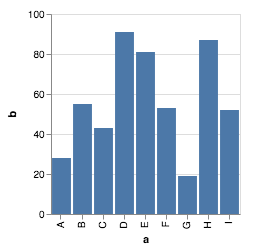
\includegraphics{figures/vis-disable-controls.png}
\caption{Without Controls}
\label{f:vis-disable-controls}
\end{figure}

Vega-Lite has a \emph{lot} of options:
for example,
we can use points and average the Y values.
(We will change the X data so that values aren't distinct in order to show this off,
because otherwise averaging doesn't do much.)
In our revised spec,
\texttt{x} is now \texttt{"nominal"} instead of \texttt{"ordinal"}
and \texttt{y} has an extra property \texttt{"aggregate"},
which is set to \texttt{"average"}
(but can be used to specify other \gref{g:aggregation-function}{aggregation functions}):

\begin{minted}{js}
    let spec = {
      "$schema": "https://vega.github.io/schema/vega-lite/v2.0.json",
      "description": "Disable control links.",
      "data": {
        "values": [
          {"a": "P", "b": 19},
          {"a": "P", "b": 28},
          {"a": "P", "b": 91},
          {"a": "Q", "b": 55},
          {"a": "Q", "b": 81},
          {"a": "Q", "b": 87},
          {"a": "R", "b": 43},
          {"a": "R", "b": 52},
          {"a": "R", "b": 53}
        ]
      },
      "mark": "point",
      "encoding": {
        "x": {"field": "a", "type": "nominal"},
        "y": {"field": "b", "type": "quantitative", "aggregate": "average"}
      }
    }
    let options = {
      ...disable controls as before...
    }
    vegaEmbed("#vis", spec, options)
\end{minted}

\figref{f:vis-aggregate-points} shows the result.

\begin{figure}
\centering
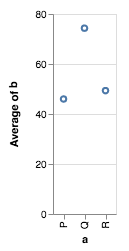
\includegraphics{figures/vis-aggregate-points.png}
\caption{Aggregating and Using Points}
\label{f:vis-aggregate-points}
\end{figure}

\section{Local Installation}\label{s:vis-vega-local}

Loading Vega from a \gref{g:cdn}{Content Delivery Network} (CDN) reduces the load on our server,
but prevents offline development.
Since we want to be able to work when we're disconnected,
let's load from local files.

Step 1 is to slim down our HTML file so that it only loads our application:

\begin{minted}{html}
<!DOCTYPE html>
<html>
  <head>
    <title>Load Vega from a File</title>
    <meta charset="utf-8">
    <script src="app.js" async></script>
  </head>
  <body>
    <div id="vis"></div>
  </body>
</html>
\end{minted}

In step 2,
we \texttt{npm\ install\ vega\ vega-lite\ vega-embed} and \texttt{require('vega-embed')} in \texttt{app.js}:

\begin{minted}{js}
const vegaEmbed = require('vega-embed')

const spec = {
  // ...as before...
}

const options = {
  // ...as before...
}

vegaEmbed("#vis", spec, options)
\end{minted}

We launch this with Parcel via our saved \texttt{npm\ run} command:

\begin{minted}{shell}
$ npm run dev -- src/vis/react-01/index.html
\end{minted}

But nothing appears when we open \texttt{http://localhost:4000} in our browser.
Looking in the browser console,
we see a message telling us that \texttt{vegaEmbed} is not a function.

What we have tripped over is something that's still painful in 2018.
The old method of getting libraries is \texttt{require},
and that's still what Node supports as of Version 10.9.0.
The new standard is \texttt{import},
which allows a module to define a default value so that \texttt{import\ 'something'} gets a function, a class, or whatever.
This is really handy, but \texttt{require} doesn't work that way.

We can either add the \texttt{-\/-experimental-modules} flag when using Node on the command line,
or rename our files with a \texttt{.mjs} extension,
both of which are annoying.
Alternatively,
we can get the thing we want by accessing \texttt{.default} during import,
or by referring to \texttt{vegaEmbed.default} when we call it.
These choices are also annoying,
but after a bit of fiddling and cursing,
we decide to make the fix as the library is loaded:

\begin{minted}{js}
const vegaEmbed = require('vega-embed').default

// ...as before...
\end{minted}

The third option is to use \texttt{import} where we can
and fix the \texttt{require} statements in the server-side code when Node is upgraded.
We can call the thing we import anything we want,
but we will stick to \texttt{vegaEmbed} for consistency with previous examples:

\begin{minted}{js}
import vegaEmbed from 'vega-embed'

// ...as before...
\end{minted}

If we do this,
the bundled file is 74.5K lines of JavaScript,
but at least it's all in one place for distribution.

\section{Exercises}\label{s:vis-exercises}

\exercise{Binned Scatterplots}

Vega-Lite can create
\href{https://vega.github.io/vega-lite/examples/circle_binned.html}{binned scatterplots}
in which the sizes of markers indicate how many values were put in each bin.
Modify the aggregating scatterplot shown above
so that values are binned in this way.

\exercise{Grouped Bar Charts}

Vega-Lite can display
\href{https://vega.github.io/vega-lite/examples/bar_grouped.html}{grouped bar charts}
as well as simple ones.
Find or create a simple data set and construct a grouped bar chart.
How impressed will your supervisor, your committee, or a future employee be
by your chosen color scheme?

\exercise{Limits of Declarative Programming}

Look at Vega-Lite's
\href{https://vega.github.io/vega-lite/examples/}{example gallery}
and identify one kind of plot or transformation you've used or seen
that \emph{isn't} included there.
Do you think this is because they just haven't gotten around to it yet,
or is there something about that plot or transformation
that doesn't lend itself to Vega-Lite's declarative model?

\exercise{Working With Arrays}

Vega-Lite is built on top of a visualization toolkit called \href{https://d3js.org/}{D3},
which includes \href{https://github.com/d3/d3-array}{a library for manipulating arrays}.
Write a small application that generates 1000 random values using \texttt{Math.random}
and reports the mean, standard deviation, and quartiles.
(You may also want to create a histogram showing the distribution of values.)

\section*{Key Points}

\begin{itemize}
\item
  Vega-Lite is a simple way to build common visualizations.
\item
  Vega-Lite is declarative: the user creates a data structure describing what they want, and the library creates the visualization.
\item
  A Vega-Lite specification contains a schema identifier, a description, data, marks, and encodings.
\item
  The overall layout of a Vega-Lite visualization can be controlled by setting options.
\item
  Some applications will use \texttt{require} for server-side code and \texttt{import} for client-side code.
\end{itemize}

